\documentclass[american]{scrartcl}
    \usepackage{babel}
    \usepackage[utf8]{inputenc} 
    \usepackage{csquotes}
    \usepackage{amsmath}
    \usepackage{amssymb}
    \usepackage{graphicx}   
    \usepackage{mathtools}
    \usepackage{tikz}

    
    \setlength{\parindent}{0em}
    \setlength{\parskip}{0.5em}

    % Bibliography and citations
    \usepackage[bibencoding=utf8, style=apa]{biblatex}
    \bibliography{ref}

    
    \title{Homework II - Advanced Game Theory }

    % \subtitle{A critical essay on the existing literature}

    \author{Andrea Titton}
    

% Commands
\newcommand{\set}[1]{\left\{#1\right\}}
\newcommand{\Real}{\mathbb{R}}
\newcommand{\abs}[1]{\left\lvert #1 \right\rvert}

% Graphs
\usetikzlibrary{positioning}
\tikzset{main node/.style={circle, draw,minimum size=1cm,inner sep=3pt},}

\begin{document}

% Title

\maketitle

\section*{Exercise 1}

\subsection*{(a)}

The graph representation of $(N, L)$ is,

\vspace{1cm}
\begin{center}
    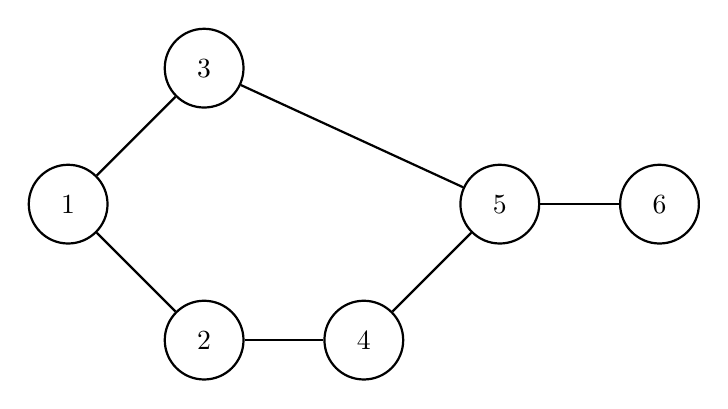
\begin{tikzpicture}[thick]
        % Nodes
        \node[main node] (1) {$1$};
        \node[main node] [below right = 1cm and 1cm of 1] (2) {$2$};
        \node[main node] [above right = 1cm and 1cm of 1] (3) {$3$};
        \node[main node] [right = 1cm of 2] (4) {$4$};
        \node[main node] [above right = 1cm and 1cm of 4] (5) {$5$};
        \node[main node] [right = 1cm of 5] (6) {$6$};
        % Paths
        \path[draw,thick]
        (1) edge node {} (2)
        (1) edge node {} (3)
        (2) edge node {} (4)
        (3) edge node {} (5)
        (4) edge node {} (5)
        (5) edge node {} (6);
    \end{tikzpicture}
\end{center}


The function $v^L$ of the Myerson restricted game is,

\begin{equation}
    v^L(S) = \sum_{T \in C_L(S)} v(T).
\end{equation}

It is non-zero only for the component of the graphs that include both $1$ and $6$, namely,

\begin{equation} \label{value_a}
    v^L(S) = \begin{cases}
        1 & \text{ if } S \in \set{\set{1, 3, 5, 6}, \set{1, 2, 3, 5, 6}, \set{1, 2, 4, 5, 6}, \set{1, 3, 4, 5, 6}, \set{1, 2, 3, 4, 5, 6}} \\
        0 & \text{ otherwise }
    \end{cases}
\end{equation}

\subsection*{(b)}

We can define the communication game $(N, v^L)$, using (\ref{value_a}). Then we can compute the Harsanyi dividends based on this game. The non-zero dividends are,

\begin{equation}
    \begin{split}
        \Delta_{v^L}(\set{1, 3, 5, 6}) &= 1 \\
        \Delta_{v^L}(\set{1, 2, 4, 5, 6}) &= 1 \\
        \Delta_{v^L}(\set{1, 2, 3, 4, 5, 6}) &= -1
    \end{split}
\end{equation}

Then we can compute the Myerson value as the Shapley value of the new coordination game,

\begin{equation} \label{myerson_complete}
    \begin{split}
        \mu_i(v, L) = f_i^S &= \sum_{T \in N(i)} \Delta_{v^L}(T) / \abs{T} \\
        \implies \mu(v, L) = f^S &= \begin{pmatrix}
            17/60 & 1/30 & 1/12 & 1/30 & 17/60 & 17/60
        \end{pmatrix}
    \end{split}
\end{equation}

\subsection*{(c)}

The new supply chain is represented by the graph,

\vspace{1cm}
\begin{center}
    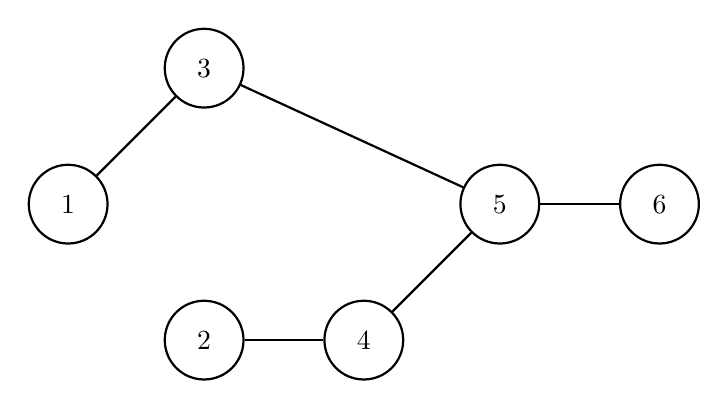
\begin{tikzpicture}[thick]
        % Nodes
        \node[main node] (1) {$1$};
        \node[main node] [below right = 1cm and 1cm of 1] (2) {$2$};
        \node[main node] [above right = 1cm and 1cm of 1] (3) {$3$};
        \node[main node] [right = 1cm of 2] (4) {$4$};
        \node[main node] [above right = 1cm and 1cm of 4] (5) {$5$};
        \node[main node] [right = 1cm of 5] (6) {$6$};
        % Paths
        \path[draw,thick]
        (1) edge node {} (3)
        (2) edge node {} (4)
        (3) edge node {} (5)
        (4) edge node {} (5)
        (5) edge node {} (6);
    \end{tikzpicture}
\end{center}

We can hence define

\begin{equation} \label{restr_v}
    v^{L^\prime}(S) = \begin{cases}
        0   & \text{ if } S = \set{1, 2, 4, 5, 6} \\
        v^L & \text{ otherwise }
    \end{cases}
\end{equation}

By repeating the procedure of (\ref{myerson_complete}), we obtain,

\begin{equation}
    \mu(v, L^\prime) = \begin{pmatrix}
        1/4 & 0 & 1/4 & 0 & 1/4 & 1/4
    \end{pmatrix}.
\end{equation}

This result is expected since in the new supply chain $2$ and $4$ become null-players.

In order to determine fairness we can check that,

\begin{equation}
    \begin{split}
        \mu_1(v, L) - \mu_1(v, L^\prime) &= \mu_2(v, L) - \mu_2(v, L^\prime) \\
        17/60 - 1 / 4 &= 1/30 - 0 \implies \text{ the fairness axiom is respected.}
    \end{split}
\end{equation}

\subsection*{(d)}

In order to compute the hierarchical outcome of node $1$ we need to set $1$ as root. The resulting directed graph $(N, L^\prime)$ can be represented as,


\vspace{1cm}
\begin{center}
    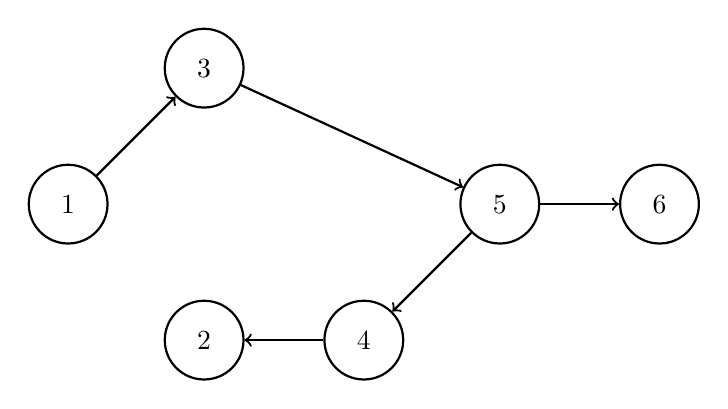
\begin{tikzpicture}[->, thick]
        % Nodes
        \node[main node] (1) {$1$};
        \node[main node] [below right = 1cm and 1cm of 1] (2) {$2$};
        \node[main node] [above right = 1cm and 1cm of 1] (3) {$3$};
        \node[main node] [right = 1cm of 2] (4) {$4$};
        \node[main node] [above right = 1cm and 1cm of 4] (5) {$5$};
        \node[main node] [right = 1cm of 5] (6) {$6$};
        % Paths
        \path[draw,thick]
        (1) edge node {} (3)
        (4) edge node {} (2)
        (3) edge node {} (5)
        (5) edge node {} (4)
        (5) edge node {} (6);
    \end{tikzpicture}
\end{center}

Using the definition of followers and subordinates, we can compute the hierarchical outcomes as,

\begin{equation}
    h^1(v, L^\prime) = \begin{pmatrix}
        v^{L^\prime}(\set{1, 3, 5, 6, 4, 2}) - v^{L^\prime}(\set{3, 5, 6, 4, 2})          \\
        v^{L^\prime}(\set{2})                                                             \\
        v^{L^\prime}(\set{3, 5, 6, 4, 2}) - v^{L^\prime}(\set{5, 6, 4, 2})                \\
        v^{L^\prime}(\set{4, 2}) - v(\set{2})                                             \\
        v^{L^\prime}(\set{5, 6, 4, 2}) - v^{L^\prime}(\set{4, 2}) - v^{L^\prime}(\set{6}) \\
        v^{L^\prime}(6)                                                                   \\
    \end{pmatrix} = \begin{pmatrix}
        1 \\ 0 \\ 0 \\ 0 \\ 0 \\ 0
    \end{pmatrix}
\end{equation}

In a similar manner,

\begin{equation}
    h^4(v, L^\prime) = \begin{pmatrix}
        0 \\ 0 \\ 0 \\ 0 \\ 1 \\ 0
    \end{pmatrix}, \hspace{0.25cm}
    h^6(v, L^\prime) = \begin{pmatrix}
        0 \\ 0 \\ 0 \\ 0 \\ 0 \\ 1
    \end{pmatrix}
\end{equation}

In order for the outcomes to belong to the $Core(v_{L^\prime})$ they need to satisfy, $\sum_{j \in N} h_j^i = v(N) = 1$ and $\sum_{j \in S}  h_j^i \geq v(S)$. The first condition is trivially satisfied since all three outcomes have one entry $1$ and all other entries $0$. The second one can be shown by using the value function (\ref{restr_v}).

First note that,

\begin{equation}
    v(S) = 1 \implies \set{1, 5, 6} \subset S.
\end{equation}

Furthermore,

\begin{equation}
    \begin{split}
        \sum_{j \in S} h_j^1 &= 1 \iff 1 \in S \\
        \sum_{j \in S} h_j^4 &= 1 \iff 5 \in S \\
        \sum_{j \in S} h_j^6 &= 1 \iff 6 \in S
    \end{split}
\end{equation}

Hence whenever $v(S) = 1$, the sum of the hierarchical outcomes needs to be one. Namely,

\begin{equation}
    \left(v(S) = 1 \implies \sum_{j \in S} h_j^i = 1\right) \implies \sum_{j \in S} h_j^i \geq v(S).
\end{equation}

\subsection*{(e)}

The link game $(L^\prime, r^{L^\prime})$ is given by the characteristic function,

\begin{equation} \label{value_r}
    \begin{split}
        \bar{E} &=
        \begin{dcases}
            \begin{rcases}
                \set{(1, 3), (3, 5), (5, 6)} \\
                \set{(1, 3), (4, 2), (3, 5), (5, 6)} \\
                \set{(1, 3), (3, 5), (5, 4), (5, 6)} \\
                \set{(1, 3), (4, 2), (3, 5), (5, 4), (5, 6)}
            \end{rcases}
        \end{dcases}\\
        r^{L^\prime}(E) &= \begin{cases}
            1 & \text{ if } E \in \bar{E} \\
            0 & \text{ otherwise }
        \end{cases}
    \end{split}
\end{equation}


The Shapley value of the link game is,

\begin{equation}
    f^{S}(L^\prime, r^{L^\prime}) = \begin{pmatrix}
        1/3 &
        0   &
        1/3 &
        0   &
        1/3
    \end{pmatrix}
\end{equation}


The associated position value is.

\begin{equation}
    \pi(v, L^\prime) = \begin{pmatrix}
        1/6 &
        0   &
        1/3 &
        0   &
        1/3 &
        1/6
    \end{pmatrix}
\end{equation}

\section*{Exercise 2}

A hierarchical outcome $h^i$ is in the $Core(N, v_L)$ if and only if,

\begin{equation*}
    \sum_{j \in E} h^i_j \geq v(E) \ \text{  and  } \
    \sum_{j \in N} h^i_j = v(N).
\end{equation*}

Entry $j$ in the hierarchical outcome can be written as,

\begin{equation} \label{hier_def}
    h^i_{j} = v(\hat{F}^i_j) - \sum_{h \in F^i_j}  v(\hat{F}^i_h).
\end{equation}

Pick a component of the graph $S \subseteq N$. Let the entry points of the component, that is, those nodes that are not followers of a node in the component, be

\begin{equation}
    I(S) = \set{h: h \notin F_j^i \ \ \forall j \in S }.
\end{equation}

Analogously, let the exit points of the component be,

\begin{equation}
    O(S) = \set{j: h \notin S \ \ \forall h \in F_j^i }.
\end{equation}

Finally let the set of middle nodes be, $M(S) = \set{j: j \in S \land j \notin I(S)\land j \notin O(S)}$. The sum of the hierarchical outcomes within a component are,

\begin{equation}
    \begin{split}
        \sum_{j \in S} h_j^i &= \sum_{j \in I(S)} h_j^i + \sum_{m \in M(S)} h_m^i + \sum_{o \in O(S)} h_o^i
    \end{split}
\end{equation}

Now notice that in the middle term in the only relevant nodes are the ones on the ``boundaries'', that is,

\begin{equation} \label{inner_simpl}
    \begin{split}
        \sum_{m \in M(S)} h_m^i &= \sum_{m \in M(S)} \left( v(\hat{F}^i_m) - \sum_{h \in F^i_m}  v(\hat{F}^i_h) \right) \\
        &= \sum_{m \in \cup_{j \in I(S)} F^i_j} v(\hat{F}^i_m) - \sum_{m: j \in O(S) \land j \in F^i_m} v(\hat{F}^i_m)
    \end{split}
\end{equation}

All terms that are not a follower of an entry node, $\cup_{j \in I(S)} F_j^i$, or are not followed by a exit node, $\set{m: j \in I(S) \land j \in F^i_m}$, are simplified since they come in first negatively in the hierarchical value entry for node $m$ and subsequently positively for the hierarchical value entry for the nodes following $m$. To illustrate this, for an $m \in M(S)$, equation (\ref{inner_simpl}) yields,

\begin{equation}
    v(\hat{F}_m^i) - \sum_{h \in F^i_m} v(\hat{F}_h^i) + \sum_{h \in F^i_m} v(\hat{F}_h^i) - \sum_{h \in F^i_m} \sum_{k \in F^i_k} v(\hat{F}_k^i) \ldots
\end{equation}

Using equation (\ref{inner_simpl}), we can rewrite,

\begin{equation} \label{component_breakup}
    \begin{split}
        \sum_{j \in S} h_j^i &= \sum_{j \in I(S)} v(\hat{F}_j^i) \underbrace{- \sum_{j \in I(S)} \sum_{h \in F_h^i}  v(\hat{F}_h^i)+
            \sum_{m \in \cup_{j \in I(S)} F^i_j} v(\hat{F}^i_m)}_{= 0} - \\ & \underbrace{- \sum_{m: j \in O(S) \land j \in F^i_m} v(\hat{F}^i_m)
            + \sum_{o \in O(S)} v(\hat{F}^i_o)}_{=0} - \sum_{h: h \in F_j^i \land h \in O(S)} v(F^i_h) \\
        &= \sum_{j \in I(S)} v(\hat{F}_j^i) - \sum_{h: h \in F_j^i \land j \in O(S)} v(F^i_h)
    \end{split}
\end{equation}

Where $\set{h: h \in F_j^i \land j \in O(S)}$ is the set of subordinates of an exit node.

We can now rewrite the union of all subordinates of an entry node as,

\begin{equation}
    \begin{split}
        \bigcup_{j \in I(S)} \hat{F}^i_j &= \bigcup_{h \in F_j^i \land j \in O(S)} \hat{F}^i_j \cup S \text{ by superadditivity } \\
        v\left( \bigcup_{j \in I(S)} \hat{F}^i_j \right) &\geq v\left( \bigcup_{h \in F_j^i \land j \in O(S)} \hat{F}^i_h \right) + v(S)
    \end{split}
\end{equation}

This implies that,

\begin{equation} \label{cond_one}
    \sum_{j \in S} h_j^i \geq v(S),
\end{equation}

for all connected components $S$.

Take now the full graph $N$. Trivially $O(N) = \emptyset$ and $I(S) = \set{i}$. Using equation (\ref{component_breakup}) and the fact that $O(N) = \emptyset \implies \set{h: h \in F_j^i \land j \in O(N)} = \emptyset$,

\begin{equation} \label{cond_two}
    \sum_{j \in N} h^i_j = \sum_{j \in I(N)} v(\hat{F}_j^i) - \sum_{h: h \in F_j^i \land j \in O(N)} v(F^i_h) = v(\hat{F}_i^i) = v(N)
\end{equation}

Results (\ref{cond_one}) and (\ref{cond_two}) show that the hierarchical outcomes of a superadditive game on a cycle-free graph are in the core.

\section*{Exercise 3}

The Harsanyi degree solution solution seems to have an advantage, as opposed to other solution like the hierarchical outcomes or the position value, in encoding the local structure of the graph. Namely, using the degree of nodes as weights to allocate the Harsanyi dividends rewards nodes that not only have large marginal contributions but also increase the number of components that are connected.

For illustration purposes consider the Harsanyi degree solution of game $(N, L)$ from Exercise 1.a,

\begin{equation}
    \phi^d(v, L) =
    \frac{1}{24} \cdot \begin{pmatrix}
        3 &
        2 &
        4 &
        2 &
        8 &
        5
    \end{pmatrix}.
\end{equation}

Such a result clearly highlights the usefulness of the measure since player $5$ is heavily rewarded for being necessary to connect $1$ and $6$. Another good property is that node $3$ is rewarded as much as $2$ and $4$ since it serves the same purpose within the graph. This property was not obtained with the Myerson value, in equation (\ref{myerson_complete}).

\section*{Exercise 4}

\subsection*{(a)}

Let $A, B \in \mathcal{F}$ and $A \cap B \neq \emptyset$. We need to show that $A \cup B \in \mathcal{F}$. Note that $B \in \mathcal{F}$ if and only if $B \subseteq M$ or $B \subseteq H$ or $B = (B \cap H) \cup M$.

The simple case where both sets are contained in either $H$ or $M$ is straight forward. Let $A, B \subseteq E \in \set{H, M}$, then

\begin{equation}
    A \cup B \subseteq E \in \mathcal{F}.
\end{equation}

% Next

Consider now the case in which, without loss of generality, $B = (B \cap H) \cup M$. Using set algebra we can rewrite,

\begin{equation} \label{gen_set}
    \begin{split}
        A \cup B &= A \cup ((B \cap H) \cup M) \ \text{ by commutativity } \\
        &= A \cup (B \cap H) \cup M \text{ by distributivity } \\
        &= (A \cup B) \cap (A \cup H) \cup M
    \end{split}
\end{equation}

Now if $A \subseteq M$, then $A \cup B = B \in \mathcal{F}$. If $A \subseteq H$, we can rewrite (\ref{gen_set}) as,

\begin{equation}
    \begin{split}
        A \cup B &= ((A \cup B) \cap H) \cup M \in \mathcal{F}.
    \end{split}
\end{equation}

Lastly, if $A = (A \cap H) \cup M$, then,

\begin{equation}
    \begin{split}
        A \cup B &= ((A \cap H) \cup \underbrace{M \cup B}_{B}) \cap \underbrace{((A \cap H) \cup M \cup H)}_{N}) \cup M \\
        &= ((A \cap H) \cup B) \cup M \\
        &= ((A \cup B) \cap H) \cup M \in \mathcal{F}
    \end{split}
\end{equation}

Hence, we have shown that,

\begin{equation}
    A, B \in \mathcal{F} \land A \cap B \neq \emptyset \implies A \cup B \in \mathcal{F}
\end{equation}

\subsection*{(b)}

By \citeauthor{brink} (\citeyear{brink}), a set of feasible coalition $\mathcal{F} \subseteq 2^N$ is the set of of connected coalitions in some (undirected) communication graph if and only if it contains the empty set, it satisfies union stability, 2-accessibility, and normality. In our case the set contains the empty set and satisfies union stability (as proven in \textbf{(a)}).

In our particular case $\mathcal{F}$ fails to satisfy 2-accessibility. Take $E = \set{1, 3, 4, 5}$. Clearly $\abs{E} \geq 2$. But,

\begin{equation}
    \begin{split}
        E \setminus \set{i} \in \mathcal{F} &\iff i = 1  \\
        &\implies \not\exists \ i, j \in E \land i \neq j: \ E \setminus \set{i}, E \setminus \set{j} \in \mathcal{F}.
    \end{split}
\end{equation}

\newpage
\printbibliography

\end{document}
